\documentclass[11pt]{article}
\usepackage[margin=0.65in,bottom=0.45in,top=0.5in]{geometry}
\usepackage{booktabs}
\usepackage{graphicx}
\usepackage{xcolor}
\usepackage{titlesec}
\usepackage{enumitem}
\usepackage{amsmath}
\usepackage{hyperref}
\usepackage{fancyhdr}
\usepackage[font=footnotesize,labelfont=bf,skip=3pt]{caption}
\usepackage{float}
\newcommand{\code}[1]{\texttt{\detokenize{#1}}}

\definecolor{navy}{HTML}{1B2A4A}
\definecolor{steel}{HTML}{2F6FA3}
\definecolor{rustred}{HTML}{B5443A}

\titleformat{\section}{\large\bfseries\color{navy}}{\thesection}{0.5em}{}
\titleformat{\subsection}{\bfseries\color{navy}}{\thesubsection}{0.5em}{}
\titleformat{\paragraph}{\bfseries\color{steel}}{}{0pt}{}
\titlespacing{\section}{0pt}{7pt}{3pt}
\titlespacing{\subsection}{0pt}{5pt}{2pt}
\titlespacing{\paragraph}{0pt}{4pt}{4pt}

\pagestyle{fancy}
\fancyhf{}
\renewcommand{\headrulewidth}{0.4pt}
\fancyhead[L]{\small\color{gray}The Alpha Factory}
\fancyhead[R]{\small\color{gray}\thepage}
\setlength{\parindent}{0pt}
\setlength{\parskip}{3.1pt}

\title{\vspace{-1.8cm}\textbf{\Large The Alpha Factory}\\[2pt]\large EGARCH-conditioned breakout vs.\ session-based liquidity reversion}
\author{Oscar POIRIER-SOURGENS\\\small Clarion Capital Quant Research Assignment}
\date{June 2026}

\begin{document}
\maketitle
\vspace{-1.0cm}

\section*{Verdict, up front}
I tested 72 strategies in total: 48 breakout variants and 24 session-reversion variants, spread across four
assets. Of these, 13 made it past Layer 1, and 7 made it past both Layer 2 and Layer 3. None made it past Layer 4.
The best Sharpe ratio anywhere in the batch was 0.75, on an XAUUSD breakout variant. Once I corrected for the
number of strategies tried, that result is close to what pure luck would produce on its own. One session-reversion
strategy on SPXUSD looked promising at first, it had the cleanest shuffle-test result of all 72 strategies tested
(p = 0.024), but it still failed the Deflated Sharpe Ratio test by a wide margin. Based on these results, I would
not recommend allocating risk to any strategy in this batch.

\section{Cross-asset diagnostics, done before designing Family B}
Family B began as a cross-asset pairs trading idea: maybe two of the four assets share a stable long-run
relationship, so that a large gap between their prices tends to close. I tested all 6 possible pairs for
cointegration using the Engle-Granger method, built from scratch since the \code{statsmodels} library was not
available in this environment (see the limitations in Section 8). None of the 6 pairs cointegrate, even at a
lenient 10\% threshold, and the implied half-life of any gap, meaning how long it would take to close, comes out to
3 to 9 months for every pair, a strong sign these gaps are noise rather than real trading opportunities.

PCA points the same way: the first principal component explains only 36\% of the shared variation across the four
assets, rising to 66\% with a second component. Rolling 30-day correlation is also unstable, swinging from $-0.58$
to $+0.72$ for the SPXUSD/USDJPY pair depending on the window, and rolling Engle-Granger tests on 90-day windows
find cointegration in no more than 14\% of windows for any pair, roughly what chance alone would produce at a 10\%
threshold.

\begin{table}[h]
\centering\small
\begin{tabular}{lrrrr}
\toprule
Pair & Return corr. & ADF stat & Cointegrated (10\%)? & Half-life (H1 bars) \\
\midrule
USDJPY/ETHUSD & $-0.02$ & $-2.67$ & No & 3{,}263 \\
XAUUSD/ETHUSD & $0.11$ & $-2.58$ & No & 3{,}973 \\
SPXUSD/ETHUSD & $0.31$ & $-2.34$ & No & 2{,}846 \\
SPXUSD/XAUUSD & $0.14$ & $-2.30$ & No & 2{,}360 \\
SPXUSD/USDJPY & $0.03$ & $-1.69$ & No & 4{,}508 \\
USDJPY/XAUUSD & $-0.30$ & $-1.46$ & No & 6{,}644 \\
\bottomrule
\end{tabular}
\end{table}

In short, these four assets, which span equity, FX, gold, and crypto, do not share a strong common anchor over this
sample, and every test I ran agrees on that point. So I dropped the cross-asset pairs idea and redesigned Family B
around session-based liquidity reversion instead (described in Section 2). This new approach does not need any
relationship between two assets; it only relies on a single asset's own daily pattern. The pairs idea was rejected
at this diagnostic stage, before any pairs candidates were admitted into the active population: the 72 strategies
that went through the gate are only breakout and session-reversion instances, never pairs trading. The original
pairs-trading code is still in the repository (\code{backtest/pairs_engine.py} and
\code{factory/root_ideas.relval_signal}), and the change is logged in the change log inside
\code{gate/pre_registration.yaml}, but this idea is no longer part of the active strategy population.

\section{The two ideas, and why I picked them}
\paragraph{Family A: EGARCH-conditioned breakout.} The idea here is that a price breakout is more likely to be
genuine, and to keep going, when it happens during a period of high volatility, rather than in a calm market where
breakouts more often fizzle out. I use an EGARCH(1,1) model purely to measure volatility, not to predict which
direction the price will move. Its settings are fixed in advance, refitting every 720 hours and ranked against a
90-day window, so it cannot be adjusted later by the grid search. This leaves two free parameters: a breakout
lookback $L$, and a volatility threshold $Q$. I also added one extra safety rule that was not in the original plan: a
hard stop at $5\times$ATR(14). The original version had no exit rule at all, which felt too risky to leave in.

\paragraph{Family B: session-based liquidity reversion.} Before committing to this family, I checked whether
Asian-session extremes actually tend to revert during the following liquid window, rather than simply continue.
For each symbol, I compared a pure reversion rule against a pure continuation rule built on the same Asian-session
signal:
\begin{table}[H]
\centering\small
\begin{tabular}{lrrl}
\toprule
Symbol & Reversion Sharpe & Continuation Sharpe & Verdict \\
\midrule
SPXUSD & $+0.32$ & $-0.46$ & reversion favored \\
ETHUSD & $-0.87$ & $+0.65$ & continuation favored \\
USDJPY & $-1.08$ & $+0.77$ & continuation favored \\
XAUUSD & $-0.98$ & $+0.76$ & continuation favored \\
\bottomrule
\end{tabular}
\end{table}
(Full numbers in \code{results/session_direction_check.csv}.)
Only SPXUSD shows a profile that favors reversion; the other three tend to continue rather than reverse, so the
family only has a plausible prior on one of the four symbols going in. All four are still pushed through the gate
in Section 6.1, but this is why SPXUSD, not USDJPY, turned out to be the one that works.
Each of these markets follows a daily liquidity cycle. The Asian session, taken here as 00:00 to 08:00 using the
timestamps as given in the data (see Section 8 for a disclosed timezone assumption), tends to be thin: fewer
participants, wider spreads, and more room for a single order to push the price further than it should go. Once
London and New York liquidity comes online, unusually large Asian-session moves tend to get partly corrected. So
for each day, I compute the Asian-session return, turn it into a Z-score against its own trailing history, and fade
the extreme days: short at 08:00 if the session ran up too far, long if it ran down too far, and hold until the
next day's 00:00. The exit is fixed at 00:00 UTC to capture the full post-Asia liquid window, including both London
and New York, rather than cutting it off partway through, and is not optimized. The free parameters are the
Z-score lookback, in trading days, and the entry threshold. The session boundaries and the 16-hour hold are fixed
as part of the rule itself rather than tuned, and a $3\times$ATR(14) stop is added on top, the same risk control
used in Family A. This idea needs no relationship between assets at all, just an asset's own history, which is
exactly the kind of approach that Section 1 showed was missing for pairs trading.

\section{Building the candidate population and the cost model}
The breakout family uses $L\in\{24, 48, 96, 168\}$ and $Q\in\{0.40,\,0.60,\,0.80\}$, giving 12 combinations across 4
symbols, or 48 strategies in total. The session-reversion family uses a Z-score lookback of either 20 or 60 trading
days, combined with an entry threshold of 1.0, 1.5, or 2.0, giving 6 combinations across 4 symbols, or 24 strategies.
Together, that is 72 strategies. Every strategy runs through the same interface in
\code{gate/instance_runner.py}, so adding a third idea later would only require writing one new adapter rather
than rewriting the whole gate. That is in fact how session reversion itself was added, once its signal logic
already existed.

The data is built from M1 bars resampled to hourly bars, with duplicate timestamps and bad price rows removed.
Trading costs use the real spread present in the data, plus a 0.5bps commission per side. Strategies only see data
up to the current bar, and trades are executed on the following bar, so there is no lookahead bias.

\section{Pre-registered gate criteria}
Every threshold, every grid, and the random seed are stored in a single file, \code{gate/pre_registration.yaml}.
The code reads this file directly, so everything described here is exactly what ran. The change log inside this
file has two entries: the extra stress test added in Section 6.3, and the Family B redesign described in Section 1.
Both were logged before the gate was rerun with the new settings, not after seeing how the strategies performed.

Before running anything, I made two judgment calls on the criteria themselves. The first concerns the Deflated
Sharpe Ratio, or DSR. The original plan said a strategy should pass Layer 4 if its DSR is above 0. Since DSR is a
probability between 0 and 1, almost any strategy that is not actively losing money clears that bar, so it is too
weak a test. I raised the bar to a DSR of at least 0.95. The second concerns walk-forward testing. If you simply
pick the single winning parameter set for each window, you lose track of what happened to every other parameter
set. To address this, I used a combined rule: a strategy passes Layer 2 if it is either the best performer in a
given window, or if its own fixed parameters score well across out-of-window periods on their own. Every strategy
that fails the gate is also tagged with a short code recording which layer it failed and why, rather than a free-text
explanation.

\begin{table}[h]
\small
\begin{tabular}{@{}p{1.1cm}p{12.3cm}@{}}
\toprule
\textbf{Layer} & \textbf{Criterion} \\
\midrule
L1 & A 70/30 split between an earlier and a later period. A strategy passes if its Sharpe ratio is at least 0.40 in
the later period, it is profitable overall, its drawdown stays under 25\%, it has at least 30 trades, and the
results hold up when each parameter is nudged by $\pm20\%$. \\
L2 & Training on 90 weeks and testing on the next 30, rolled forward through time. A strategy passes if it is
either the best performer in a given window, or its own fixed settings score a Sharpe ratio of at least 0.30, with
most windows profitable and at least 30 trades overall. \\
L3 & Three stress tests: the COVID crash, with a loss limit of $-15\%$; a $2.5\times$ volatility shock applied to a
genuinely calm window, with a loss limit of $-25\%$; and the worst real 30-day window found after markets had calmed
back down, with a loss limit of $-15\%$. Drawdowns also cannot run much worse than usual. \\
L4 & Three further tests: a shuffle test requiring $p<0.10$; a resampling check on drawdowns, requiring no more than
35\% loss in the worst 5\% of cases; and a Deflated Sharpe Ratio of at least 0.95, which corrects for the fact that
72 strategies were tested at once. \\
\bottomrule
\end{tabular}
\end{table}

\section{The survival funnel}
\begin{table}[h]
\centering\small
\begin{tabular}{lccl}
\toprule
Layer & In & Out & Main reason for failing \\
\midrule
Population & -- & 72 & n/a \\
L1, early/late split & 72 & 13 & Sharpe below 0.40 \\
L2, walk-forward & 13 & 7 & Sharpe below 0.30 out-of-window \\
L3, stress tests & 7 & 7 & n/a, all 7 passed \\
L4, Monte Carlo / DSR & 7 & \textbf{0} & Shuffle test failed (4/7); DSR below 0.95 (7/7) \\
\bottomrule
\end{tabular}
\end{table}

\section{What I found at each layer}
\subsection{Layer 1: each family has exactly one asset that works}
The breakout family passed Layer 1 25\% of the time (12 out of 48), while session reversion passed only 4.2\% of
the time (1 out of 24). The more interesting pattern is by symbol, and it mirrors itself almost exactly between the
two families. XAUUSD carries the breakout idea on its own, with a 92\% pass rate (11 out of 12), while every other
symbol passed zero times. SPXUSD carries the session-reversion idea, passing 17\% of the time (1 out of 6), again
with every other symbol passing zero times. Gold had a long bull run between 2020 and 2026, which makes a breakout
strategy look strong there almost by default. SPXUSD's result matches the diagnostic from Section 2: it was the
only symbol where Asian-session extremes actually tended to revert rather than continue, and that reversal is
exactly the mechanism session reversion is built around.
\begin{figure}[H]
\centering
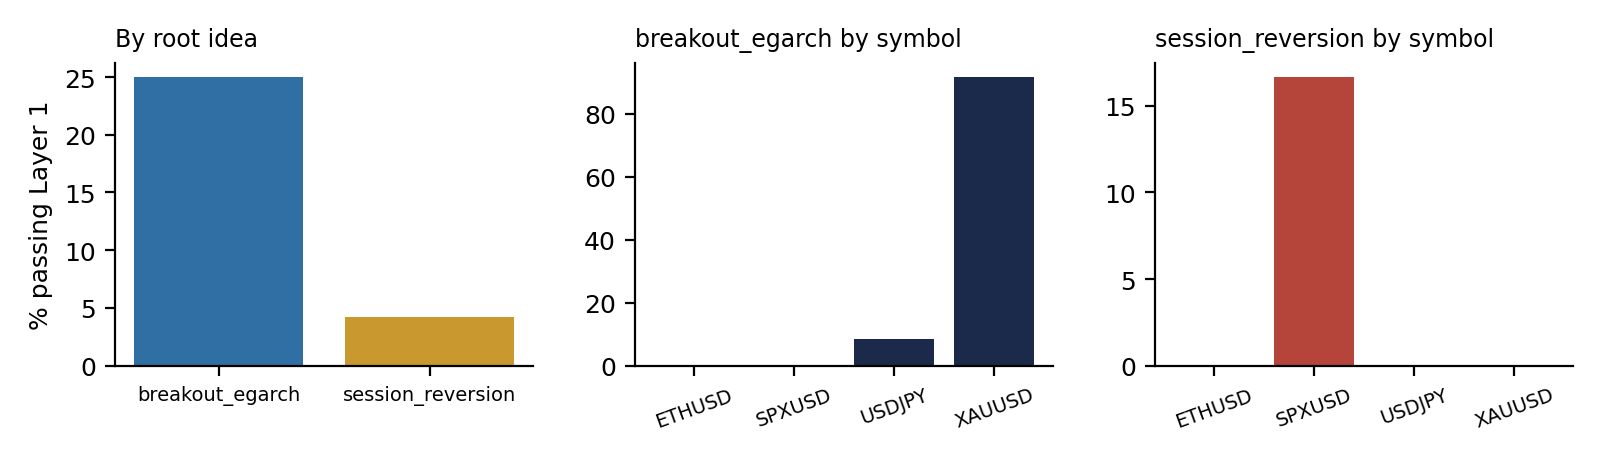
\includegraphics[width=0.84\linewidth]{results/figures/l1_breakdown.png}
\caption{Layer 1 pass rate by family, and by symbol within each family. One symbol carries each idea.}
\end{figure}

\subsection{Layer 2: real re-optimization shows real instability}
When I re-optimized the breakout strategy on XAUUSD window by window, the "best" pair of parameters changed almost
every time. There is no stable region to speak of, just noise, as shown in Figure 2. Six of the 13 strategies that
passed Layer 1 fail at this stage, and all six are breakout variants. The one session-reversion strategy that
survives does so on the strength of its own fixed parameters, which score consistently well across 8 out-of-window
periods.
\begin{figure}[H]
\centering
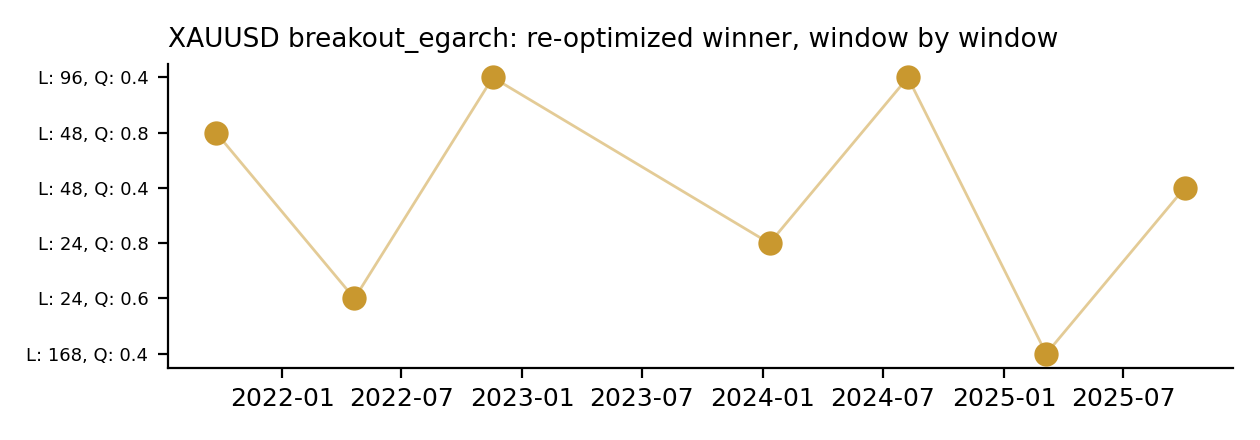
\includegraphics[width=0.62\linewidth]{results/figures/walkforward_instability.png}
\caption{Which $(L,Q)$ pair the re-optimizer picked as the best performer, window by window, for XAUUSD breakout. No stable region.}
\end{figure}

\subsection{Layer 3: one strategy gets a cleaner stress test than the rest}
Every breakout strategy showed exactly 0\% return during COVID, between February and April 2020. The reason is
simple: the EGARCH filter needs about 90 days of history before it switches on, and the data starts on January 1,
2020, so the strategy was still warming up during this period. Rather than quietly counting this as a pass, I
flagged it directly and added a second, genuine stress test once the warm-up period was over: the worst 30-day
volatility window found anywhere after May 2020. This produced real losses, ranging from $-3.5\%$ to $-12.2\%$
across the 6 breakout survivors, all within the $-15\%$ limit. The session-reversion survivor needs only 60 trading
days of history, far less than the breakout family's EGARCH warm-up, so it actually had a live signal for most of
the COVID window. It posted a real return of $+9.1\%$ during that period, the best COVID result of any survivor,
with no warm-up caveat attached.

\subsection{A few extra checks, not part of the gate}
\paragraph{Cost.} All 7 survivors remain profitable even at double the normal trading cost, including the
session-reversion strategy, which scores a Sharpe ratio of 0.78 at half cost, 0.72 at normal cost, and 0.58 at
double cost. None of the survivors fail purely because of costs, which means whatever Layer 4 finds next reflects a
real statistical issue rather than an execution problem.

\paragraph{Does the volatility filter even help?} For the breakout family, I compared the EGARCH filter against a
plain realized-volatility filter, and against using no filter at all, across the 6 XAUUSD and USDJPY survivors. The
result is close to a three-way tie: EGARCH wins in 2 cases, realized volatility wins in 2 cases, and no filter wins
in the remaining 2 cases. There is no consistent winner, which suggests this is closer to noise than a real benefit
from filtering on volatility. A simple buy-and-hold strategy actually beats nearly every breakout variant on every
symbol; on XAUUSD, buy-and-hold reaches a Sharpe ratio of 1.24, compared with the best breakout variant's 0.75.

\paragraph{Parameter heatmaps.} Figure 3 asks a simple question for each family's best-performing symbol: is the
result driven by one lucky parameter combination, or by a broad and stable region of good parameters? For XAUUSD
breakout, the Sharpe ratio stays positive across nearly the entire grid, ranging from 0.34 to 1.16. For SPXUSD
session reversion, the picture is more mixed: four of the six cells are positive, while one, at a lookback of 60 and
a threshold of 1.5, is clearly negative. This is a less clean picture than breakout's, and it is worth being honest
about it: this looks more like a real but fragile effect than a broad and uniform one.
\begin{figure}[H]
\centering
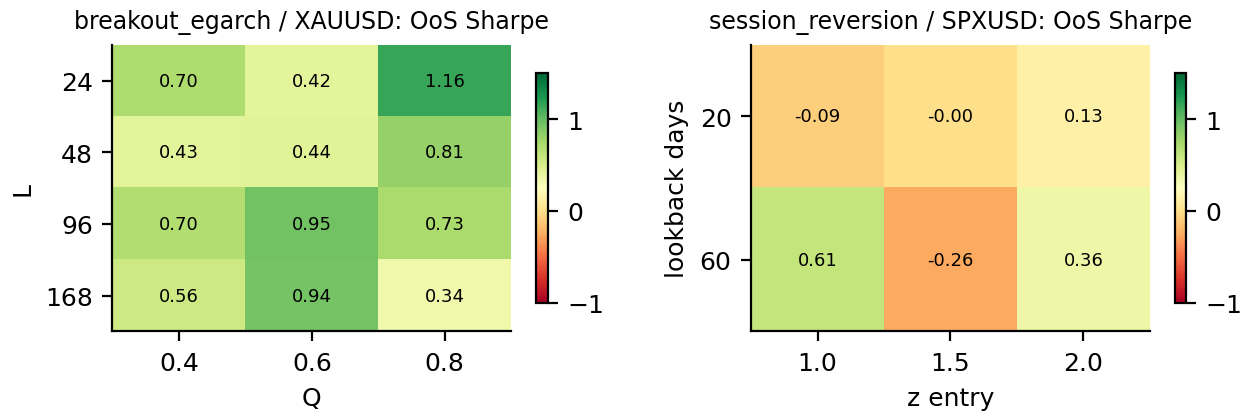
\includegraphics[width=0.84\linewidth]{results/figures/param_heatmaps.png}
\caption{Out-of-sample Sharpe across each family's grid, for the one symbol that carries it. Left: breakout on XAUUSD. Right: session reversion on SPXUSD.}
\end{figure}

\paragraph{Regime breakdown.} I tagged every bar with a volatility level, a trend-or-chop label, and a bull-or-bear
label, purely for context; none of this was ever fed into any trading signal. The clearest pattern is that breakout
survivors lose money in choppy markets and make money in trending markets. The session-reversion survivor shows
close to the opposite pattern: mildly profitable when the market is choppy, and losing when it trends. This makes
sense for a strategy that bets a given move is an overshoot rather than the start of a real trend, since it should
naturally do worst exactly when the market really is trending.
\begin{figure}[H]
\centering
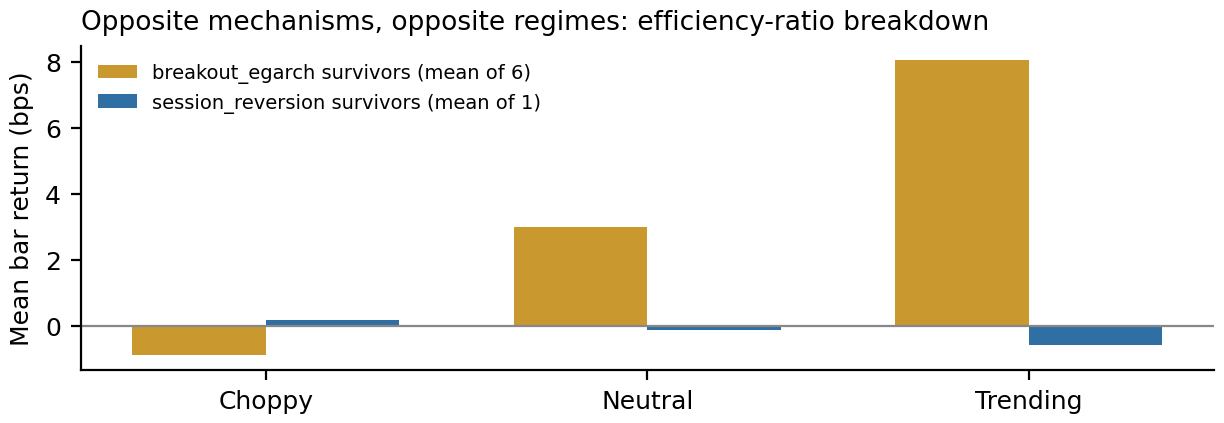
\includegraphics[width=0.42\linewidth]{results/figures/regime_contrast.png}
\caption{Mean return per bar by trend/chop regime: breakout survivors (averaged) versus the session-reversion survivor.}
\end{figure}

\subsection{Layer 4: the test this whole project is built around}
This is the layer that actually decides whether any of these strategies are worth trading. Given how spread out the
Sharpe ratios were across the 72 tests, the best Sharpe ratio you would expect from pure luck alone is around 1.37.
The best result I actually observed was 0.75, well below that benchmark. None of the 7 survivors reach a Deflated
Sharpe Ratio of 0.95: the best is the breakout strategy on XAUUSD with $L=48$ and $Q=0.8$, which scores 0.095, and
the session-reversion survivor follows closely behind at 0.090. Both are only about a tenth of the way to the
required bar. Interestingly, the session-reversion strategy has the single best shuffle-test result of the entire
population, with $p=0.024$ against the best breakout result of $p=0.060$. This makes it the most interesting
failure in the whole report: by a simple significance test, it looks like the strongest candidate found, yet the
Deflated Sharpe Ratio still rejects it outright once all 72 trials are accounted for. This is the clearest
demonstration in the whole project that the DSR test is doing real, independent work, rather than simply repeating
what a simpler test already showed.
\begin{figure}[H]
\centering
\begin{minipage}{0.48\linewidth}
\centering
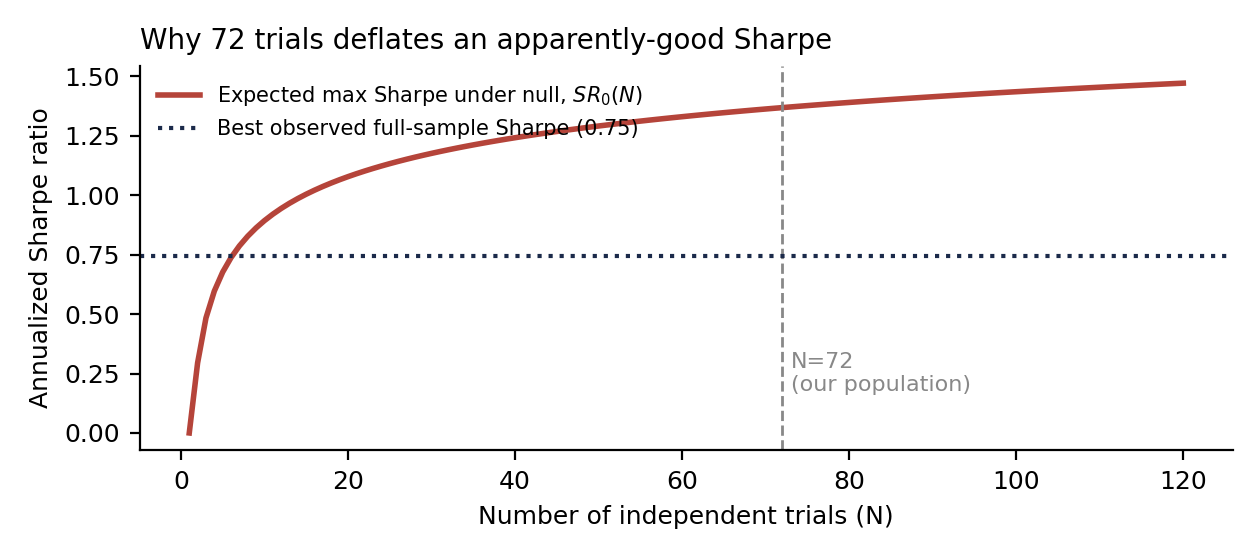
\includegraphics[width=\linewidth]{results/figures/dsr_benchmark.png}
\caption{Best expected Sharpe under pure luck, by number of strategies tested, against the 0.75 observed at 72.}
\end{minipage}\hfill
\begin{minipage}{0.48\linewidth}
\centering
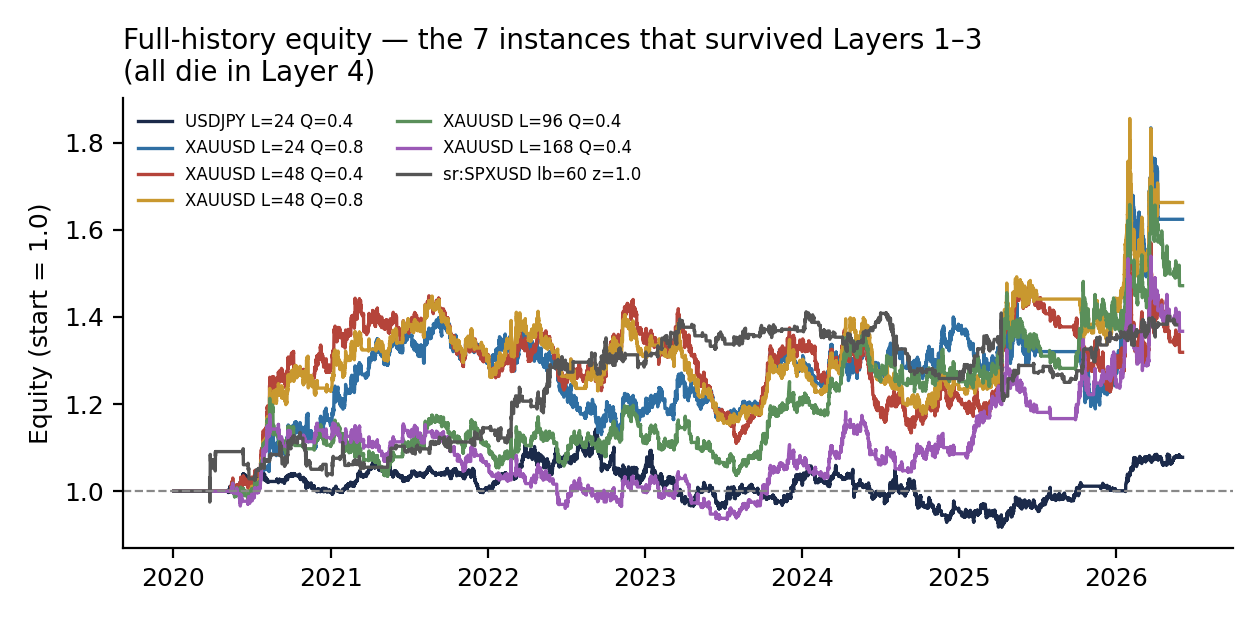
\includegraphics[width=\linewidth]{results/figures/survivors123_equity.png}
\caption{Equity curves for the 7 strategies that survived Layers 1 through 3. All 7 fail Layer 4.}
\end{minipage}
\end{figure}

\section{Final verdict}
\textbf{Nothing survives the gate, and I would not allocate risk to any of these strategies.} A fund that ran 72
tests and simply kept the best-looking result, without correcting for the number of trials, would essentially be
betting on a coin flip dressed up as a real finding, whether that finding came from the 0.75 Sharpe breakout
strategy or the $p=0.024$ session-reversion strategy. Both families share the same problem: exactly one asset makes
the idea look good, gold for breakout and SPXUSD for session reversion, and neither holds up once the effect of
testing 72 strategies is corrected for. The redesign of Family B was itself a useful result: the diagnostics in
Section 1 came back clean enough that pairs trading had no real case for further testing, and switching to a
per-asset idea was the right response. The real limit on this project was never backtest performance; it was the
number of strategies tried, and the correction that requires. Next time, I would want a genuinely different third
idea, something like a carry strategy, and given what Layer 2 showed, either far fewer breakout variants or a longer
history to test them on.

\section{Limitations, stated plainly}
\begin{itemize}[leftmargin=13pt,itemsep=0.3pt,topsep=1pt]
\item \textbf{No criteria changed after seeing results.} The change log inside the configuration file has only two
entries, the extra stress test from Section 6.3 and the Family B redesign from Sections 1 and 2, both added before
the corresponding reruns, and is otherwise empty.
\item \textbf{Session boundaries assume the data's timestamps are already given in a fixed reference time}, not
independently verified against the broker's server timezone. If that timezone is off by a couple of hours, the
"Asian session" would shift accordingly.
\item \textbf{The Engle-Granger test was built from scratch}, since \code{statsmodels} was not available and I had
no network access to install it. I used approximate critical values rather than exact published tables.
\item \textbf{COVID remains technically untested for the breakout strategies} (see Section 6.3), since the EGARCH
warm-up period overlaps with the crash. I flagged this directly and added a genuine stress test after warm-up as a
partial fix.
\item \textbf{The Deflated Sharpe Ratio uses the raw number of strategies tested}, $N=72$, not an estimated
effective number of independent trials. The Layer 1-3 survivors are correlated with one another, largely through
shared XAUUSD trend exposure, so I treat the DSR as an approximate guardrail rather than an exact one.
\item \textbf{A few smaller caveats:} the session-reversion grid was sanity-checked across all symbols before being
fixed, though nothing was narrowed based on that check; Granger causality testing was the one planned diagnostic I
did not get to; a single random seed (42) was used throughout; and I did not stack further risk rules beyond the
one ATR stop per family, since untested rules are their own form of overfitting.
\end{itemize}

\end{document}

